% !TeX spellcheck = es_AR
\documentclass[10pt, a4paper]{article}


\usepackage[utf8]{inputenc}
\usepackage[spanish]{babel} % separación silábica en castellano
\usepackage{hyphsubst}

%\usepackage[paper=a4paper, margin=2cm]{geometry} % especifico márgenes manualmente
\usepackage{a4wide} % margenes un poco más anchos

\usepackage{microtype} % saca warnings de underfull boxes
\usepackage{fancyhdr} % encabezado y pie de página
\usepackage{lastpage} % para que muestre la última página en footer

% Comandos para figuras, graficos, tikz, etc.
\usepackage{tikz}
\usepackage{epsfig}
\usepackage{graphicx}
\usepackage{float}
\usepackage{caption}
\usepackage{subcaption}
\usepackage{svg}

% Comandos para teoremas, etc.
\usepackage{amsmath}
\usepackage{amsthm}
\usepackage{amssymb}

\usepackage[backend=biber]{biblatex}

\addbibresource{recursos.bib}

\usepackage{algorithm}
\usepackage[noend]{algpseudocode}
\usepackage{csquotes}

\usepackage{hyperref}
\hypersetup{
    colorlinks=true,
    linkcolor={blue!80!black},
    filecolor=magenta,
    urlcolor=cyan,
    pdftitle={TPF Orga2 2c2021},
    pdfpagemode=UseNone,
    citecolor=blue,
}

\pagestyle{fancy} % Acomodo el encabezado y pie de página.
\lhead{Organización del Computador II}
\setlength{\headheight}{12pt}
\rhead{Segundo Cuatrimestre 2021}
\cfoot{\thepage /\pageref{LastPage}}

\begin{document}

\hfill 
\includegraphics[scale=0.5]{imgs/logo_dc.jpg}~\\[0.25cm]

\begin{center}
    \textbf{\Large Ray Tracer en C vs. x64 ASM + SIMD}\\[1cm]
    {\large Jonathan Teran Carballo}\\[0.15cm]
    Universidad de Buenos Aires\\[0.15cm]
    \texttt{jonathan.nerat@gmail.com}\\[1cm]
\end{center}

\begin{abstract}
    En este trabajo implementaremos un Ray Tracer en C y en x64 ASM utilizando extensiones SIMD para
    comparar la performance de ambos. El mismo es capaz de renderizar mallas de triangulos, utiliza
    KD Trees para optimizar la detección de colisiones, y permite asignar materiales a cada objeto
    de una escena.
\end{abstract}


\hrulefill
\tableofcontents
\clearpage

\section{Introducción} \label{sec:introduccion}

Las arquitecturas x86 y x64 incluyen un modelo de ejecución llamado SIMD
(\textit{Single Instruction Multiple Data}), que consiste en realizar una
operación sobre un conjunto de datos en una sola instrucción. Este modelo
resulta útil a la hora de procesar contenido multimedia, donde se aplican
algoritmos sobre un conjunto de datos que sigue el mismo formato. A diferencia
del modelo SISD (\textit{Single Instruction Single Data}), este modelo permite
acelerar la ejecución de estos algoritmos paralelizando la manipulación de los
datos de entrada.

Para medir las mejoras de performance que ofrece este modelo, implementaremos 2
Ray Tracers: uno en C y otro en x64 ASM utilizando SIMD. Compararemos tiempos de
ejecución al generar escenas con distintos tipos de objetos, materiales, y
cantidades.

La idea de este proyecto como trabajo final fue inspirada en el trabajo de
Martín Mongi \cite{rtmartin}. Además, las implementaciones están basadas en una
implementación anterior en C++ \cite{RayTracerCpp}, que a su vez está basado en
las guías de Shirley \cite{RTIOW}. En la sección \ref{sec:diferencias}
discutiremos que diferencias existen entre este trabajo, el trabajo de Mongi y
la implementación original en C++.


%LTeX: language=es-AR
\section{Diferencias con otras implementaciones y trabajos} \label{sec:diferencias}

A lo largo de este trabajo, haremos referencia a las otras implementaciones para
remarcar ciertas diferencias. Es por esto que llamaremos RTMongi, RTC++, RTC y
RTASM a cada una respectivamente.

\subsection{Trabajo de Mongi}

En este trabajo se modifican / agregan las siguientes características:

\paragraph{Objetos} Nuevos objetos, como: planos, cubos y mallas de triángulos
usando archivos \texttt{.obj} en formato STL. Las luces se definen como materiales, y no
como objetos.

\paragraph{Materiales} El color de los objetos no es explícito, sino que se
especifica como un material: lambertiano (color difuso), metálico, dieléctrico, y
un material especial para emitir luz.

\paragraph{Archivo de salida} Se permite parametrizar el \textit{max depth}
(cantidad de veces que un rayo puede rebotar en objetos de la escena) y
\textit{samples per pixel} (cantidad de rayos aleatorios que se mandan dentro
del área correspondiente a cada pixel).

\paragraph{Cámara de escena} Se permite parametrizar la posición del origen, la
dirección en la que apunta, dirección ``arriba'', amplitud del ángulo de
\textit{field of view}, y la apertura de la lente.

\paragraph{Optimización} Nueva estructura KDTree para optimizar el cálculo de
intersecciones entre un rayo y muchos objetos (por ejemplo, en una malla de
triángulos)

\paragraph{Imagen} Para escenas similares, los resultados difieren por la
iluminación.

\subsection{Implementación original en C++}

La implementación en C++ (es decir, RTC++) hace uso de propiedades de la
programación orientada a objetos, como herencia, polimorfismo, etc. Para este
proyecto, se simplificó el código para mejorar la \textit{performance} en la
implementación en ASM (RTASM).

En un principio, lo ideal era simular herencia y polimorfismo con estructuras y
punteros a funciones para facilitar la implementación en C (RTC), pero termino
siendo contraproducente, ya que la diferencia de performance entre C y ASM
resulto ser insignificante. En su lugar, se simplificaron las estructuras de
objetos y materiales para que compartan una estructura \textit{header} común
(herencia) con un campo \texttt{type} que determine el tipo concreto
(polimorfismo).

Por otro lado, como RTC++ hace uso de estructuras de la librería estándar de C++
(\texttt{vector} y \texttt{smart\_ptr}, entre otros), se implementaron
estructuras básicas similares que proveen solamente la funcionalidad que se usa
en este proyecto.

Operaciones como el parsing de la entrada, el overhead inicial de la creación de
objetos y el overhead final en el que se liberan los recursos no se consideran
para medir el rendimiento, y, por lo tanto, se implementan en C.


\section{Ray Tracing} \label{sec:ray-tracing}

El \textit{Ray Tracing} es un algoritmo de renderizado en el que una imagen se
crea identificando los objetos que contribuyen a cada pixel (\textit{image-order
rendering}). Dada una escena con objetos tridimensionales, se puede obtener una
imagen de la misma lanzando rayos desde un origen (cámara) hacia una ventana, y
trazando la trayectoria de los mismos para ver sobre que objetos / materiales
incidió (Figura \ref{fig:rt-camera-window-scene}).

\begin{figure}[H]
    \centering
    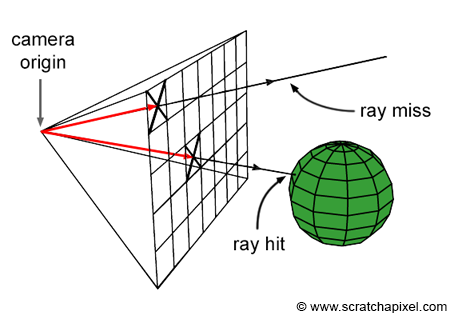
\includegraphics[width=.7\textwidth]{imgs/rt-camera-throwing-rays-into-scene.png}
    \caption{Cámara lanzando rayos por una ventana hacia una escena}
    \label{fig:rt-camera-throwing-rays-into-scene}
\end{figure}

En esta situación, la imagen final es el resultado de muchas variables:

\begin{itemize}
    \item Cámara: posición, dirección, inclinación, apertura de la lente,
        distancia de foco.
    \item Objetos: ubicación, tamaños, formas, etc.
    \item Materiales (de cada objeto): tipos (lambertiano, metálico, etc),
    color, reflexión, refracción, etc.
    \item Archivo de salida: Dimensiones, \textit{spp}, \textit{max depth}.
\end{itemize}

A continuación explicaremos como cada uno influye en la imagen final.

\subsection{Cámara} \label{ssec:rt-camera}

Como ya se mencionó, el origen de los rayos estará dado por la cámara. No
solamente por su posición, sino también por su orientación (es decir, que
dirección es la de ``arriba''), la apertura de la lente y la distancia de foco.

Para poder controlar el ``nivel de enfoque'' de la imagen, la implementación
simula la lente de la cámara usando como verdadero origen de los rayos a un
disco. La apertura es el diámetro de la lente, y la distancia de foco
es la distancia entre el disco y el plano de foco.

\begin{figure}[H]
    \centering
    
\includegraphics[width=.7\textwidth]{imgs/rt-camera-rays-through-lens.png}
    \caption{Lente y plano de foco}
    \label{fig:rt-camera-plano-foco}
\end{figure}

Los rayos se lanzarán desde un punto aleatorio de la lente, hacia distintos
puntos en el plano de foco (dependiendo del pixel que se este calculando).
Mientras más chico sea el diámetro de la lente, y más cerca esté el plano de
foco del objetivo, más nítida será la imagen. Por el contrario, si la lente es
muy grande, o el plano de foco se encuentra lejos del objetivo, la imagen se
verá más borrosa.

\subsection{Objetos}

Los objetos son cuerpos del espacio tridimensional que pueden colisionar con los
rayos y en consecuencia, modificar la trayectoria de los mismos y finalmente  la
imagen. Dependiendo del material de su superficie, estos pueden reflejar o
refractar los rayos, y cambiar el color de cada pixel. En este trabajo se
implementaron 4 objetos

\begin{itemize}
    \item Esferas
    \item Planos
    \item Cubos
    \item Triángulos
\end{itemize}

Cada objeto es definido por una función que indica si un rayo colisiona o no con
el mismo (\texttt{hit}). Además, esta función retorna (en caso de que haya
colisión) detalles de como se dio la misma: el punto de intersección, la normal
de la superficie en ese punto, el material del objeto, etc.

Por ejemplo, la función \texttt{hit} de un plano devuelve verdadero si el rayo
\textbf{no} es paralelo al plano (suponiendo que el rayo y el plano no se
superponen). Por otro lado, para una esfera la función devuelve verdadero si el
rayo ``pasa'' lo suficientemente cerca del origen (radio de la esfera).

Formalmente, representaremos a un rayo como un par
$\left\langle P, D \right\rangle$, donde $P$ es el punto de origen y $D$ es la
dirección. De esta forma, podemos describir cada punto del rayo $R(t) = P + tD$.
La función \texttt{hit} de un objeto (e.g. \textsc{\texttt{ObjectHit}}) recibirá
como parámetros:

\begin{itemize}
    \item El objeto, para saber sus coordenadas y dimensiones
    \item El rayo
    \item $t_{min}$ y $t_{max}$: el rango de valores de $t$ (del rayo) a
        considerar. Por ejemplo, no consideramos colisiones con $t < 0$ porque
        se encuentran detrás de la cámara y no aparecen en la imagen final
\end{itemize}

Y retornará dos valores:

\begin{itemize}
    \item Un booleano, para indicar si hay intersección o no
    \item Un diccionario con los datos de la colisión, si corresponde
\end{itemize}

Como vimos, la implementación de cada función \texttt{hit} puede ser muy
diferente dependiendo de la forma y las propiedades de cada objeto, así que
exploraremos cada uno por separado.

\subsubsection{Plano}

Un plano está dado por un origen $O$ y una normal $N$. Para decidir si un rayo
$R(t) = P + tD$ interseca con el plano, bastará con ver que no sean paralelos.
El punto de intersección (en particular, el parámetro $t$ del rayo) se puede
despejar de la ecuación del plano:

\begin{align*}
    ((P + tD) - O) \cdot N &= 0 \\
    (tD \cdot N) + (P - O) \cdot N &= 0 \\
    t(D \cdot N) &= (O - P) \cdot N \\
    t &= \frac{(O - P) \cdot N}{D \cdot N} \\
\end{align*}

\begin{algorithm}[H]
\begin{algorithmic}[1]
\Function{PlaneHit}{$Plane, Ray, t_{min}, t_{max}$}{$\rightarrow (hit, record)$}
    \State $O, N \gets Plane$ \Comment{Descomponemos en origen y normal}
    \State $P, D \gets Ray$ \Comment{Descomponemos en origen y dirección}
    \If {$N \perp D$} \Comment{Rayo y plano son paralelos}
        \State \Return (False, NIL)
    \EndIf
    \State $t \gets ((O - P) \cdot N)/(D \cdot N)$

    \If {$\lnot (t_{min} \le t \le t_{max})$} \Comment{Punto fuera del rango permitido}
        \State \Return (False, NIL)
    \EndIf

    \State $record \gets$ ($t$, $N$, \dots) \Comment{Datos de la intersección}
    \State \Return (True, $record$)
\EndFunction
\end{algorithmic}
\caption{Algoritmo \textit{hit} para planos}
\label{alg:plane-hit}
\end{algorithm}

El algoritmo \ref{alg:plane-hit} encapsula estas reglas. Devuelve un par $(hit,
record)$ donde $hit$ es un booleano que indica si hubo intersección, y $record$
contiene los datos de la misma (como la ``distancia'' desde el origen del rayo
$t$, o la normal del plano de intersección $N$), o \texttt{NIL} si no hubo
intersección.

\subsubsection{Esferas}

Para representar una esfera usamos un punto $C$ para representar el centro, y un
radio $r$. La ecuación de los puntos $Q=(x, y, z)$ de la superficie de una
esfera esta dada por:

\begin{align*}
    (x - C_x)^2 + (y - C_y)^2 + (z - C_z)^2 &= r^2 \\
    (Q - C) \cdot (Q - C) = r^2
\end{align*}

Si $Q = R(t) = P + tD$, podemos reemplazarlo en la ecuación y obtener una
ecuación cuadrática en $t$.

\begin{align*}
    (P + tD - C) \cdot (P + tD - C) &= r^2 \\
    t^2 D \cdot D + 2tD \cdot (P - C) + (P - C) \cdot (P - C) - r^2 &= 0
    \label{eq:cuad-esfera}
\end{align*}

Esta función puede tener 0, 1 o 2 raíces, dependiendo de si el rayo intersecta o
no con la esfera, y en cuantos puntos lo hace. Si la función no tiene raíces, no
existe $t$ que satisfaga la ecuación de la esfera, y por lo tanto, no hay
intersección. Si la función tiene 1 raíz, el rayo intersecta a la esfera en
\textbf{un} único punto, y es tangente a la superficie de la misma. Por otro
lado, si la función tiene 2 raíces, el rayo atraviesa a esfera y la intersecta
en 2 puntos, uno de entrada y uno de salida.

Para decidir si el rayo intersecta o no, podemos calcular el discriminante y ver
si es negativo (no intersecta) o no.

\begin{algorithm}[H]
\begin{algorithmic}[1]
\Function{SphereHit}{$Sphere, Ray, t_{min}, t_{max}$}{$\rightarrow (hit, record)$}
    \State $C, r \gets Sphere$ \Comment{Descomponemos en centro y radio}
    \State $P, D \gets Ray$ \Comment{Descomponemos en origen y dirección}
    \State $a \gets D \cdot D$
    \State $b \gets 2D \cdot (P - C)$
    \State $c \gets (P - C) \cdot (P - C) - r^2$
    \State $disc \gets b^2 - 4ac$

    \If {$disc < 0$}
        \State \Return (False, \texttt{NIL})
    \EndIf

    \State $t \gets (-b - \sqrt{disc} / 2a)$
    \If {$t < t_{min} \lor t_{max} < t$}
        \State $t \gets (-b + \sqrt{disc} / 2a)$
        \If {$t < t_{min} \lor t_{max} < t$}
            \State \Return (False, \texttt{NIL})
        \EndIf
    \EndIf

    \State $N \gets P + tD - C$ \Comment{Normal al plano de la intersección}
    \State $record \gets$ ($t$, $N$, \dots) \Comment{Datos de la intersección}
    \State \Return (True, $record$)
\EndFunction
\end{algorithmic}
\caption{Algoritmo \textit{hit} para esferas}
\label{alg:sphere-hit}
\end{algorithm}

\subsubsection{Cubos}

La forma más directa de implementar cubos es utilizando planos para representar
cada cara. Para simplificar la implementación, solo representaremos cubos
alineados a los ejes de coordenadas del espacio, de forma tal que basta con dar
las coordenadas de 2 vertices opuestos para determinar su posición y tamaño.

Sobre cada uno de estos vertices ubicamos 3 planos con normales sobre cada eje,
con dirección opuesta al otro vértice, de forma que los 6 planos encapsulen el
volumen del cubo.

% TODO: incluir imagen de lo descripto anteriormente

Debido a que los planos son infinitos y estan sobre cada eje del espacio,
cualquier rayo intersecará con al menos 2 planos del cubo. Para decidir si
alguna de estas intersecciones corresponde a alguna cara del cubo, tenemos que
verificar que el punto se encuentre dentro del volumen del mismo. Para esto
usamos las coordenadas de los 2 vertices que definen al cubo: cada coordenada
del punto de intersección debe estar entre las coordenadas correspondientes de
los vertices.

\begin{algorithm}[H]
\begin{algorithmic}[1]
\Function{CubeHit}{$Cube, Ray, t_{min}, t_{max}$}{$\rightarrow (hit, record)$}
    \State $vmin \gets Cube.vmin$ \Comment{Obtenemos los vertices del cubo}
    \State $vmax \gets Cube.vmax$
    \State $faces \gets Cube.faces$

    \State $hitAnyFace \gets$ False
    \State $closestSoFar \gets \infty$
    \State $cubeRecord \gets$ NIL

    \For {$face \in faces$} \Comment{Cada cara es un plano}
        \State {$(faceHit, faceRecord) \gets$ PlaneHit($face, Ray, t_{min}, closestSoFar$)}
        \State {$insideBox \gets$ puntoEntreVertices($faceRecord.p, vmin, vmax$)}

        \If {$faceHit \land insideBox$}
            \State {$hitAnyFace \gets$ True}
            \State {$closestSoFar \gets faceRecord.t$}
            \State {$cubeRecord \gets faceRecord$}
        \EndIf
    \EndFor

    \State \Return ($hitAnyFace, cubeRecord$)
\EndFunction
\end{algorithmic}
\caption{Algoritmo \textit{hit} para cubos}
\label{alg:box-hit}
\end{algorithm}

En el algoritmo \ref{alg:box-hit}, $hitAnyFace$ es \texttt{True} si y solo si el
rayo $Ray$ interseca a alguna cara del cubo y lo hace dentro de las coordenadas
definidas por los limites del mismo ($vmin$ y $vmax$). En ese caso, se setea
$closestSoFar$ para ignorar las proximas intersecciones que podrían quedar detrás
de la más cercana a la camara, y se guarda el registro de la interseccion en
$cubeRecord$.

\subsubsection{Triangulos}

Nuevamente podemos utilizar lo que conocemos sobre planos para definir un
triangulo. Al definir el triangulo con 3 puntos, definimos tambin el plano sobre
el que se encuentra. Para acomodarnos a la representacion que adoptamos para los
planos, podemos usar alguno de los vertices como origen, y calcular la normal
como el producto vectorial de los vectores que inciden sobre el origen.

% TODO: incluir grafico que ilustre esto.

Al igual que hicimos con el cubo, primero calcularemos el punto de interseccin
entre el rayo y el plano, y luego verificaremos que el punto se encuentre entre
los vertices del triangulo para determinar si el rayo intersecta o no con el
mismo. Para verificar esto, tenemos que definir una convención para indicar que
cara del triangulo es la ``visible'' (es decir, en que sentido apunta la normal
del plano). Sean $P_1$, $P_2$ y $P_3$ los vertices del triangulo, entonces llamamos
cara ``visible'' a la cara en la que estos vértices aparecen en sentido anti-horario.

Si sabemos que los vertices aparecen en cierto orden, detectar un punto dentro de
la superficie del triangulo consiste en verificar que el punto se encuentra ``dentro''
para cada borde. Es decir, sea $P$ un punto en el plano del triangulo, si:

\begin{itemize}
    \item $(P_2 - P_1) \times (P - P_1)$ apunta en el sentido de la normal,
    \item $(P_3 - P_2) \times (P - P_2)$ apunta en el sentido de la normal, y
    \item $(P_1 - P_3) \times (P - P_3)$ apunta en el sentido de la normal
\end{itemize}

significa que $P$ esta ``dentro'' del triangulo para cada borde.

\begin{algorithm}[H]
\begin{algorithmic}[1]
\Function{TriangleHit}{$Triangle, Ray, t_{min}, t_{max}$}{$\rightarrow (hit, record)$}
    \State $P_1, P_2, P_3 \gets Triangle$ \Comment{Obtenemos los vertices del triangulo}
    \State $normal \gets (P_2 - P_1) \times (P_3 - P_1)$
    
    \If {$normal \perp Ray.dir$}
        \State \Return (False, NIL) \Comment{Si el rayo es paralelo al plano, no hay hit}
    \EndIf

    \State $t \gets ((P_1 - Ray.origin) \cdot normal) / (Ray.dir \cdot normal)$
    \If {$\lnot (t_{min} \le t \le t_{max})$} 
        \State \Return (False, NIL)
    \EndIf

    \State $P \gets Ray.at(t)$ \Comment{Punto de intersección}
    \State $dentroBorde1 \gets normal \cdot ((P_2 - P_1) \times (P - P_1)) > 0$
    \State $dentroBorde2 \gets normal \cdot ((P_3 - P_2) \times (P - P_2)) > 0$
    \State $dentroBorde3 \gets normal \cdot ((P_1 - P_3) \times (P - P_3)) > 0$


    \If {$dentroBorde1 \land dentroBorde2 \land dentroBorde3$}
        \State $record \gets (t, p, normal, \dots)$
        \State \Return (True, $record$)
    \EndIf

    \State \Return (False, NIL)
\EndFunction
\end{algorithmic}
\caption{Algoritmo \textit{hit} para triangulos}
\label{alg:triangle-hit}
\end{algorithm}

Se puede comprobar que el sentido de dos vectores es el mismo al ver el signo de
su producto interno, ya que $A \cdot B = \vert A \vert \vert B \vert
\cos{\theta}$, donde $\theta$ es el angulo entre $A$ y $B$. En este caso,
$\theta$ o bien es 0 y $\cos{0} = 1$, o bien es 180 y $\cos{180}=-1$.

\subsection{Materiales}

Los materiales están asociados a cada objeto y se encargan de darle color a una
escena. Cada material puede emitir / atenuar luz y reflejar / refractar
rayos. En este trabajo, se implementaron 4 tipos:

\begin{itemize}
    \item Luz Difusa
    \item Lambertiano
    \item Metal
    \item Dieléctrico
\end{itemize}

Cada material implementa 2 métodos: \texttt{Scatter} (atenuar / dispersar) y
\texttt{Emit} (emitir):

\begin{itemize}
    \item \texttt{Scatter} recibe 3 parámetros: el material ($M$) sobre el que
        incide el rayo, el rayo en cuestión ($R_{in}$), y la metadata de la
        colisión ($rec$) que se dio sobre el objeto al que esta asociado el
        material. Devuelve 3 valores: \textit{did\_scatter} que indica si el
        material puede dispersar rayos en el punto de intersección,
        \textit{R\_{out}} el rayo dispersado en caso de que el anterior sea
        \texttt{TRUE}, y $A$ la atenuación del color que produce el material.
    \item \texttt{Emit} solamente recibe el material $M$ y retorna el color que
        emite el mismo.
\end{itemize}

Estos métodos serán llamados por cada rayo que se genere desde la cámara.
\texttt{Scatter} se encarga de dirigir cada rayo en cada colisión, hasta llegar
a un material que no disperse más (\textit{did\_scatter} en \texttt{False}), o
hasta que se supere el \textit{max depth} de la imagen.

Por la naturaleza de los materiales que se eligieron, Luz Difusa solamente emite
luz, y el resto solamente atenúa luz  y refleja / refracta los rayos que
reciben. A continuación describiremos como se implementa estos métodos, y en los
casos en los que se omita alguno se toma por defecto que \texttt{Emit} devuelve
un color negro \texttt{\#000000} (es decir, no emite luz), y que
\texttt{Scatter} devuelve \texttt{(False, NIL, NIL)} (es decir, ni atenúa ni
dispersa).

\subsubsection{Luz Difusa}

Para crear este material solo necesitamos un color $A$, que será el valor que se
devuelva al llamar al método \texttt{Emit} sobre el mismo.

\begin{algorithm}[H]
\begin{algorithmic}[1]
\Function{DiffuseLightEmit}{$Light$}{$\rightarrow A$}
    \State \Return $Light.A$
\EndFunction
\end{algorithmic}
\caption{Algoritmo \textit{Emit} para Luz Difusa}
\label{alg:diffuse-light-emit}
\end{algorithm}

\subsubsection{Lambertiano}

Un material difuso o lambertiano se caracteriza por verse uniformemente
iluminado de todas las direcciones. Si bien posee un color propio $A$, también
toma parte de los colores de su entorno para formar el color final de la imagen.

\begin{algorithm}[H]
\begin{algorithmic}[1]
    \Function{LambertianScatter}{$Lambertian, r_{in}, rec$}{$\rightarrow
    (did\_scatter, A, R_{out})$}

    \State $scatterdir \gets rec.normal +$ (vector random en esfera unitaria)

    \If {$scatterdir \approx \vec{0}$}
        \State $scatterdir \gets rec.normal$
    \EndIf

    \State $r_{out} \gets \left \langle rec.p, scatterdir \right \rangle$
    \State \Return (True, $Lambertian.A$, $r_{out}$)
\EndFunction
\end{algorithmic}
\caption{Algoritmo \textit{Scatter} para material Lambertiano}
\label{alg:lambertian-scatter}
\end{algorithm}

Para simular el aporte uniforme de todo el entorno, en el algoritmo
\ref{alg:lambertian-scatter} tomamos como referencia la normal al plano de
intersección $rec.normal$ y le sumamos un vector random $v$ en la esfera
unitaria (es decir, $v \in \mathbb{R}^3, \vert v \vert = 1$). Puede ocurrir que
$rec.normal \approx -v$, lo cual resulte en un $scatterdir \approx 0$. En ese
caso, simplemente tomamos $scatterdir = rec.normal$.

\subsubsection{Metal}

Por otro lado, los materiales metálicos están caracterizados por reflejar muy
bien los rayos, dependiendo de que tan ``pulido'' esté el mismo. Vamos a
parametrizar un material metálico nuevamente con un color $A$, y con un valor de
\textit{fuzziness} $f \in [0, 1]$. Si $f=0$, los rayos se reflejan perfectamente
sobre la superficie, y para $f>0$, se le suma algo de aleatoriedad al rayo de
salida, cuyo aporte incrementa con $f$.

\begin{algorithm}[H]
\begin{algorithmic}[1]
    \Function{MetalScatter}{$Metal, r_{in}, rec$}{$\rightarrow
    (did\_scatter, A, R_{out})$}

    \State $d \gets r_{in}.dir$
    \State $n \gets rec.normal$
    \State $reflected \gets d - 2 (d \cdot n) n $

    \If {$reflected \cdot n \le 0$} 
        \State \Return (False, NIL, NIL)
    \EndIf

    \State $scatterdir \gets reflected + Metal.f \times$ (vector random en esfera
    unitaria)

    \State $r_{out} \gets \left \langle rec.p, scatterdir \right \rangle$
    \State \Return (True, $Metal.A$, $r_{out}$)
\EndFunction
\end{algorithmic}
\caption{Algoritmo \textit{Scatter} para material metálico}
\label{alg:metal-scatter}
\end{algorithm}

Como vemos en el algoritmo \ref{alg:metal-scatter}, la aleatoriedad la provee un
vector random en la esfera unitaria. En caso de que el rayo reflejado no se
encuentre del lado de la cara de la superficie ($reflected \cdot n \le 0$), el
material no dispersa el rayo y devuelve \texttt{(False, NIL, NIL)}.

\subsubsection{Dieléctrico}

Los materiales dielectricos son aquellos que al recibir rayos de luz, son
capaces de separarlos en un rayo que se refleja, y otro que se refracta. Si bien
nuestra representación solo permite un rayo de salida, simularemos este
comportamiento reflejando y refractando rayos en cada punto de un objeto de
manera aleatoria.

\begin{figure}
    \centering
    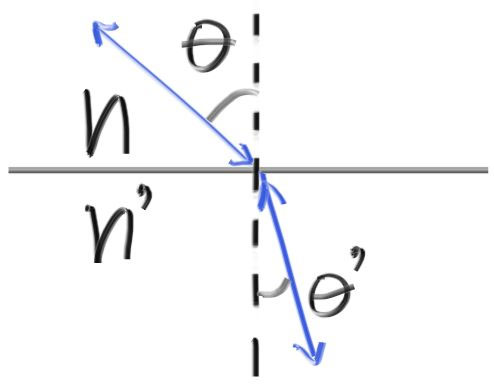
\includegraphics[width=.7\textwidth]{imgs/refraction.jpg}
    \caption{Ley de Snell}
    \label{fig:snell-law}
\end{figure}

Ya vimos como calcular el rayo reflejado, así que veremos como calcular el
refractado. Así como un rayo se refleja al entrar en contacto con una
superficie, la refracción se da en la frontera entre 2 materiales con indices de
refracción $\eta$ y $\eta'$ (ver figura \ref{fig:snell-law}). Si el rayo viaja
por un material ($\eta$), y llega a la frontera con otro material ($\eta'$), el
angulo de ``entrada'' en el primer material $\theta$ y el angulo de ``salida'' en el
segundo material $\theta'$ están relacionados por la ley de Snell:

\[
    \eta \sin \theta = \eta' \sin \theta'
\]

Suponiendo que conocemos $\eta$ y $\eta'$ (uno es el índice del material, y el
otro podemos asumir que es el índice del aire), y como además conocemos $\theta$
(el angulo con el que un rayo incide sobre una superficie respecto de la
normal), podemos calcular $\sin \theta'$ despejando de la ecuación:

\[
    \sin \theta' = \frac{\eta}{\eta'} \sin \theta
\]

El rayo refractado que se encuentra del otro lado de la frontera es $R'$, y se
puede descomponer en $R'_{\perp}$ perpendicular a la normal, y
$R_{\parallel}$ paralela a la normal: $R' = R'_{\perp} + R'_{\parallel}$.

Se puede probar que cada componente se calcula como:

\begin{align*}
    R'_{\perp} &= \frac{\eta}{\eta'}(R + (-R \cdot n) n) \\
    R'_{\parallel} &= - \sqrt{1 - \vert R'_{\perp} \vert^2} n
\end{align*}

Y finalmente, el rayo refractado se puede calcular con el algoritmo
\ref{alg:refract}.

\begin{algorithm}[H]
\begin{algorithmic}[1]
    \Function{Refract}{$R$, $n$, $i$}{ $\rightarrow R'$}

    \State $cos_{\theta} = \min\{-R \cdot n, 1.0\}$
    \State $R'_{\perp} = i (R + cos_{\theta} n)$
    \State $R'_{\parallel} = - \sqrt{\vert 1 - \Vert R'_{\perp} \Vert ^ 2 \vert} n$

    \State \Return $R'_{\perp} + R'_{\parallel}$
\EndFunction
\end{algorithmic}
\caption{Algoritmo para refractar un rayo $R$ sobre una superficie con normal
$n$ y relación de indices de refracción $i = \eta / \eta'$}
\label{alg:refract}
\end{algorithm}

Si usáramos éste algoritmo para definir \texttt{DielectricScatter} y calcular el
nuevo rayo, obtendríamos imágenes poco realistas, ya que los materiales
dieléctricos no siempre refractan los rayos. Por ejemplo, si el radio entre los
indices de refracción es mayor a 1, la refracción no es posible:

\[
    \sin \theta' = \frac{\eta}{\eta'} \cdot \sin \theta = i \cdot \sin \theta
\]

Como $\sin \theta' \in [0, 1]$, si $i \cdot \sin \theta > 1$, entonces no existe valor
de $\theta'$ que satisfaga la ecuación.

Además, los materiales dieléctricos son capaces de reflejar dependiendo del
ángulo sobre el que incide el rayo. Si bien existe una ecuación para determinar
ésto, podemos usar la aproximación de Schlick \cite{schlicksapprox} como una
alternativa simple y que para nuestro caso de uso alcanza. La misma se basa en
el uso de una propiedad llamada \textit{reflectance} que se calcula usando el
coseno del ángulo de incidencia y la relación entre los índices de refracción.

\begin{algorithm}[H]
\begin{algorithmic}[1]
\Function{Reflectance}{$\cos_{\theta}$, $i$}{ $\rightarrow R'$}
    \State $r \gets \frac{1 - i}{1 + i}$
    \State \Return $r^2 + (1-r^2) (1 - \cos_{\theta})^5$
\EndFunction
\end{algorithmic}
\caption{Calculo de la \textit{reflectance} de un rayo que incide con un ángulo
cuyo coseno es $\cos_{\theta}$, y con un radio de refracción $i = \eta / \eta'$}
\label{alg:reflectance}
\end{algorithm}

El algoritmo \ref{alg:reflectance} calcula este valor. Lo que luego se pide en
la aproximación es que sea mayor que un valor aleatorio entre $[0, 1]$.

\begin{algorithm}[H]
\begin{algorithmic}[1]
\Function{DielectricScatter}{$Dielectric, r_{in}, rec$}{$\rightarrow
    (did\_scatter, A, R_{out})$}
    \State $r \gets Dielectric.ir$
    \If {hit in $rec$ was front face}
        \State $r \gets Dielectric.ir^{-1}$
    \EndIf
    \State $u \gets normalized(r_{\text{in}}.direction)$
    \State $\cos_{\theta} \gets \min(1, -u \cdot rec.normal)$
    \State $\sin_{\theta} \gets \sqrt{1 - \cos_{\theta}^2}$

    \If {$r \sin_{\theta} > 1$ \textbf{or} reflectance($\cos_{\theta}, r$) $>$ (random in
    [0, 1])}
        \State $dir \gets$ reflect($u$, $rec.normal$)
    \Else
        \State $dir \gets$ refract($u, rec.normal, r$)
    \EndIf

    \State \Return (True, $Dielectric.albedo$, $\langle rec.point, dir \rangle$)
\EndFunction
\Function{reflect}{$v$, $n$}{$\rightarrow v'$}
    \State \Return $v - 2 (v \cdot n) n$
\EndFunction
\end{algorithmic}
\caption{Algoritmo \textit{Scatter} para material dieléctrico}
\label{alg:dielectric-scatter}
\end{algorithm}


% IDEAS
% - Comparar C vs ASM:
%   - Imágenes: deberian ser identicas salvo randomness
%   - Velocidad: ASM debería ser más rápido
% - Comparar con Mongi (C vs C y ASM vs ASM):
%   - Imágenes para el mismo setup, como son las imagenes generadas (visualmente)
%   - Velocidad: usar los mismos casos de prueba del informe de Mongi para
%     comparar los tiempos de ejecucion en esos casos
% - Comparar con implementacion original:
%   - Imágenes para el mismo setup (deberian ser identicas, salvo randomness)
%   - Velocidad: debería ser mas rápido

\section{Experimentación}

En esta sección pondremos a prueba a ambos Ray Tracer, y los compararemos entre
sí en diferentes escenarios para ver si efectivamente el uso de instrucciones
SIMD mejora el rendimiento de los mismos.

Todos los experimentos se corrieron en una notebook HP 14-dk1003dx, que cuenta
con una CPU AMD Athlon Silver 3050U de 2.3GHz, 1MB de cache L2, y 16GB de RAM.
El sistema corre Arch Linux, y utiliza la versión 6.7.5 de linux. Los binarios
en C y en ASM se compilaron con GCC v13.2.1 y con NASM v2.16.01 respectivamente.

\subsection{Diferencia entre implementaciones}

En este primer experimento, generaremos imágenes para escenas similares usando
las distintas implementaciones que tenemos a disposición: el ray tracer de
Mongi, el original en C++, y el desarrollado en ASM (el que está hecho en C
genera exactamente las mismas imágenes). La motivación es tener una idea general
de como se diferencian los ray tracers, y además una medida del tiempo que tarda
cada uno en generar la imagen de la escena.

Por la diferencia en cómo esta implementado cada uno, esperamos que el de Mongi
sea el más rápido, y el original en C++ el más lento. La implementación de Mongi
usa una simplificación para el cálculo del color, en vez de ``rebotar'' el rayo
por la escena hasta llegar a una fuente de luz y combinar los aportes de todas
las superficies, en la primer intersección se calcula el aporte de cada fuente
de luz con la superficie.

\begin{figure}
    \centering
    \begin{subfigure}[b]{0.45\textwidth}
        \centering
        \includegraphics[width=\textwidth]{../images/impl_diffs/mongi-sphere.png}
        \caption{Implementación de Mongi}
        \label{fig:yellow-sphere-mongi}
    \end{subfigure}
    \hfill
    \begin{subfigure}[b]{0.45\textwidth}
        \centering
        \includegraphics[width=\textwidth]{../images/impl_diffs/asm-sphere.png}
        \caption{Implementación en ASM}
        \label{fig:yellow-sphere-asm}
    \end{subfigure}
    \hfill
    \begin{subfigure}[b]{0.45\textwidth}
        \centering
        \includegraphics[width=\textwidth]{../images/impl_diffs/cpp-sphere.png}
        \caption{Implementación original en C++}
        \label{fig:yellow-sphere-cpp}
    \end{subfigure}

    \caption{Escena de una esfera amarilla sobre una superficie gris}
    \label{fig:yellow-sphere}
\end{figure}

En la figura \ref{fig:yellow-sphere} podemos ver las imágenes generadas. La de
Mongi (\ref{fig:yellow-sphere-mongi}) es claramente distinta por lo que ya
explicamos anteriormente, se puede ver como tanto el ángulo de incidencia, como
la distancia de la intersección a la luz afectan a su aporte en la imagen,
haciendo que algunas partes se vean más oscuras. Por otro lado, las
implementaciones en ASM (\ref{fig:yellow-sphere-asm}) y en CPP
(\ref{fig:yellow-sphere-cpp}) generan imágenes muy parecidas, y más iluminadas
que en la primer imagen.

La diferencia de color que se puede apreciar entre éstas últimas se debe a cómo
están iluminadas. En ASM usamos un plano a cierta altura para que simule una luz
solar, mientras que en C++ los rayos que no colisionan con ningún objeto toman
un color predeterminado que depende de su dirección.

Los tiempos de ejecución los obtenemos realizando 10 mediciones y tomando el
promedio. Usamos el comando `time` que se puede encontrar en la mayoría de
distribuciones de Linux. El tiempo CPU es el tiempo que el programa estuvo
ejecutando, mientras que el Real es el tiempo real que transcurrió desde que
empezó la ejecución hasta que termino (puede incluir esperas de IO,
manejo de interrupciones, etc.)

\begin{itemize}
    \item Mongi:
        \begin{itemize}
            \item CPU: 328.4 ms
            \item Real: 365.3 ms
        \end{itemize}
    \item ASM:
        \begin{itemize}
            \item CPU: 4326.8 ms
            \item Real: 4361.8 ms
        \end{itemize}
    \item C++:
        \begin{itemize}
            \item CPU: 14986.5 ms
            \item Real: 15052.3 ms
        \end{itemize}
\end{itemize}

Como podemos ver, los resultados concuerdan con nuestras suposiciones iniciales.
Mongi es casi 13 veces más rápido que ASM, y ASM 3.5 veces más rápido que C++.

Si bien la diferencia es sustancial, es importante recordar que los ray tracer
en ASM y C++ pueden parametrizar opciones como \texttt{spp} y
\texttt{max\_depth}, mientras que el de Mongi los tiene fijados en 1 por
definición. Si corremos nuevamente ASM pero con un \texttt{spp=1} y
\texttt{depth=5}, podemos obtener un tiempo de ejecución de 350 ms sacrificando
la calidad de la imagen.


\subsection{Tiempos de ejecución con escena preparada para distintas
resoluciones}

Inspirado en el experimento realizado por Mongi en su trabajo, compararemos los
tiempos de ejecución de las implementaciones en C y ASM para una misma escena,
pero variando la resolución de la imagen de salida.

% generar una escena usando todos los recursos posibles (objetos, materiales,
% meshs, etc.), y medir los distintos tipos de tiempos

\subsection{Tiempos de ejecución por tipo de objeto para distintas cantidades}

% generar escenas por cada tipo de objeto que contengan solo ese tipo, y variar
% la cantidad de objetos de la escena, y ver la variación de tiempo por cada
% uno.

\subsection{Tiempos de ejecución por tipo de material para distintas cantidades}

% idem pero por cada tipo de material. Usar esferas ya que son más simples y asi
% las escenas tienen cierta uniformidad.

\subsection{Variación de depth vs. spp para una escena preparada}

% Ver como varía la imagen para distintos depth y spp, y elegir una
% configuración óptima que no sacrifique mucha calidad de imagen


\newpage
\section{Resultados y Conclusión} \label{sec:conclusion}

En este trabajo reescribimos en C un ray tracer inicialmente hecho en C++, y
luego en ASM haciendo uso de instrucciones SIMD para mejorar la performance del
mismo.

La mejora obtenida (calculada como la relación entre $t_C/t_{ASM}$), ronda entre
5 y 7, es decir, RTASM es entre 5 y 7 veces más rápido que RTC, dependiendo de
la escena que se utilice. Este rango se debe a que nuestra implementación hace
uso de números aleatorios en muchos aspectos de la generación de la imagen, como
la generación de distintos rayos para un mismo pixel, o la reflexión/refracción
de rayos en materiales dieléctricos, entre otros.

Si bien la reescritura de código C en ASM puede resultar difícil en un principio
si no es familiar, es innegable que los beneficios en performance realmente lo
valen. En este caso, obtuvimos un resultado similar al trabajo de Mongi
\cite{rtmartin}, cuya implementación con SIMD fue 6 veces más rápida que la
implementación en C.

Las operaciones que utilizamos en este trabajo simplemente paralelizaron el
cálculo de operaciones básicas entre vectores, como la suma o la resta. También
se hicieron cálculos más complejos, como el producto interno o el producto
vectorial, que simplificaron una operación que suele tomar muchas instrucciones
en una sola. Teniendo en cuenta que nuestra implementación fue realmente una
escritura de otro existente, y no fue hecha desde cero con la intención de
aprovechar instrucciones SIMD, resulta interesante pensar en que mejora
podríamos lograr reescribiendo nuevamente los algoritmos.

% Conclusiones extras sobre como se diferencia con Mongi y como se podría
% mejorar la performance
%
% Una de las principales diferencias con RTMongi, y que también puede ser el
% origen de una nueva mejora en la performance, tiene que ver con la iluminación.
% Por ahora, nuestro Ray Tracer calcula los colores de los materiales haciendo
% ``rebotar'' el rayo hasta que impacte con otro material emisor de luz. Por otro
% lado, RTMongi le asigna un color a cada objeto, y calcula el color final con la
% intensidad, y el ángulo con el que incide la luz sobre la superficie de impacto.
% 
% Podríamos incluir esta lógica en los casos en los que un rayo se pierde en el
% vacío, o cuando se alcanza el \texttt{max\_depth} de la imagen. En ese caso, en
% lugar de asignarle un color negro al rayo (como hacemos ahora), podríamos
% recorrer todos los objetos con materiales luminosos y acumular el aporte que
% realiza cada uno. Esto nos permitiría obtener imágenes con buena iluminación,
% incluso con un \texttt{max\_depth=1}, lo cual por el momento no es posible.


\newpage

\printbibliography

\end{document}
